%
% sample.tex
% $Id: sample.tex,v 1.1 2006/03/18 00:21:36 johnh Exp johnh $
%
% File is renamed to sensys-full.tex to reflect the twists made to use sensys-proc.cls.
% 

% The default of sigplan-proc-varsize is 9pt, indented paragraphs (acm style)
% For Sensys or other 10pt conference, use the 10pt option
%\documentclass{sigplan-proc-varsize}
% options:
%\documentclass[9pt]{sigplan-proc-varsize}
%\documentclass[nocopyrightspace,10pt]{sigplan-proc-varsize-sensys-abstract}

\documentclass[10pt]{sensys-proc}

% % hack to avoid the ugly ACM paragraph definition
% % => can't leave blank line after this
% (remove comment for this hack)
% \renewcommand{\paragraph}[1]{\vskip 6pt\noindent\textbf{#1 }}

\usepackage{graphicx}
\usepackage{balance}
\usepackage{comment}

\numberofauthors{3}

\author{
%
% The command \alignauthor (no curly braces needed) should
% precede each author name, affiliation/snail-mail address and
% e-mail address. Additionally, tag each line of
% affiliation/address with \affaddr, and tag the
%% e-mail address with \email.
\alignauthor Andrej Balas \\
        \affaddr{Msc. Software Development Design}\\
        \affaddr{IT University Copenhagen}\\
       \email{bala@itu.dk}
\alignauthor Nikos Grigoriadis \\
        \affaddr{Msc. Software Development Design}\\
        \affaddr{IT University Copenhagen}\\
    \email{ngri@itu.dk}
\alignauthor Hao Wu \\
        \affaddr{Msc. Software Development Design}\\
        \affaddr{IT University Copenhagen}\\
    \email{hawu@itu.dk}
}

\title{Pervasive Computing Assignment 1 - LoRa Based Plant Monitoring}

\begin{document}

\maketitle

\begin{abstract}

In this assignment we explored usage of a LoPy sensor node with an antenna and an extension board in the context of smart agriculture. The sensor node was programmed through micropython and used LoRa as the communication protocol to communicate the sensor results. We chose the Chirp soil sensor, as it measures light, soil moisture and temperature simultaneously. Through sample experiments we determined some key decisions to be made regarding energy usage of IoT devices. 
\bigskip
\end{abstract}
\section{Sensor choice}
Since the idea is to keep our plants alive, we have to somehow measure the environmental conditions the plants are surrounded by. Every plant has its specific demands so it can grow. Some plants need more light than the others, some need less water, and some can't survive unless they are in a warm place. In order to keep our plants happy and growing, we will take care that all their demands are satisfied. Using the temperature, moisture and light sensors, we will make sure that our plants are receiving enough water, light and are held in a right-heated place. Those are primar, but sufficient measures to maintain our plants.
\bigskip
\section{Sampling rate and communication}
Plants are more durable beings than humans, which means they won't be permanently damaged if we forget to water them for a day or two. If we expose them to some extreme temperatures, we might harm them, but those are really extraordinary situations. As far as light is concerned, plants are used to have day and night time, so sudden lack of light won't harm them either. Only long lack of light can cause the plant to wither. Consequently, there is no need for the frequent sampling interval.
At first, we set our program to send data to the server every minute, just out of curiosity. We wanted to check the measurements after specific events like watering the plant or turning the light on and off. However, it's not necessary to question the conditions so often, so the plan is to set the sampling interval to half an hour.
\bigskip
\section{Packet reception rate}
The reception rate is very good. In the implementation with the sampling interval of one minute, there were just some occasional absences of data. The errors were so rare that we could just ignore them. However, if we receive our data every half an hour, or even more rare, an absence of data would mean much more significant flaw.
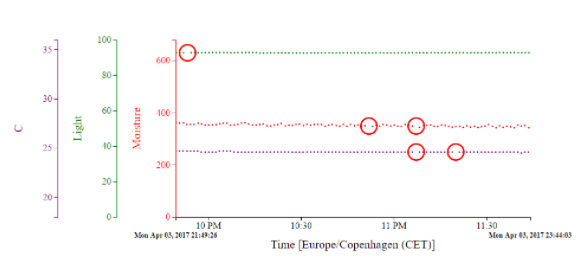
\includegraphics[height=1.7in]{./Images/figure1}
\bigskip
\section{Theoretical power consumption model}
Can you make a power consumption model based on the LoPy data sheet and
your implementation?
To create a power consumption model, we must list all the possible components that draw power. In our case  the LoPy board, its antenna and its attached sensor chip require power. Using the data sheets available for the components we found that the current at 5.5V for the components were:
\begin{itemize}
  \item LoPy Wifi: 12mA (5uA on standby)
  \item LoPy LoRa: 15mA (10uA on standby)
  \item Chirp sensor: 4.5mA (1.1mA on standby) 
\end{itemize}

In total that adds up to 31.5mA or 0.0315A when it is active and approximately 0.0011A when it is in deep sleep or on standby. 

Power consumption is calculated by multiplying the current with the voltage.
 Which means theoretically our device requires an average of 0.17 watts when active and 0.007 watts on standby.
\bigskip
\section{Power measurements of deployed device}
Ideal power consumption models never quite manifest in reality due to various factors such as resistance, temperature, entropy, etc. 

To calculate our device's actual power consumption we powered it through a USB multimeter. Due measurement inconsistencies, our results fluctuated between: 
\begin{itemize}
  \item Volts (Min-Max): 4.8-5.1V
  \item Amperes (Min-Max): 0.08-0.11A 
  \item Watts (Min-Max): 0.384-0.561W 
\end{itemize}
\bigskip
\section{Battery needs}
If we were to design a battery to power the device autonomously for a month, we first assume there is 30 days in a month, and therefore 720 hours in a month. 

Conservatively if we assume that our node is drawing a current on the high end of our actual ampere measurement (110mA). A battery would need to be 110*720 or 79200 mAh large to power our node autonomously for a month. 
\bigskip
\section{Energy harvesting}
As IoT devices, particularly in smart agriculture, need to be deployed outside the range of conventional power grids, having energy harvesting options on these devices dramatically increases their usability.
 
In our particular device we are using, the most logical energy harvesting technique would be to use solar energy panels since the plant should be exposed to a daylight. If we have a plant that doesn't need much of a daylight, we might use small windmills as an extra electricity source. Similarly, plants are very often used in gardens where we can have fountains, rills or even a waterfalls, which opens the possibility  of using water mills.
\bigskip
\section{Energy saving improvements}
Since the biggest energy consumers in our device are the wireless antenna and LED lamp, we should consider not using them, or in the case that we have to, use them only when an offline solution will not suffice. Without using the wireless, our device would be pretty poor. The fact that we can follow our plant's environmental status and thus also the plant itself using the internet, is the primary feature of our device. 

However an option would be to put the wireless technologies to a sleep state programmatically, and awake them only when they send the data. This way, we would save energy, prolonging the device's battery life. Another viable option is to reduce the frequency of data sending to an amount that is still representative of the plant?s needs. We can send the sensor data even less than one time per hour, and we should be provided with enough information about our plants. Although the latter option depends on the particular needs of the plants used with the device. 
\bigskip
\balance
\bibliographystyle{abbrv}
\bibliography{sigproc}  % sigproc.bib is the name of the Bibliography in this case
\end{document}
